\documentclass[conference]{IEEEtran}
\IEEEoverridecommandlockouts
\usepackage{cite,amsmath,amssymb,graphicx,booktabs,url}
\usepackage{tikz}
\usetikzlibrary{arrows.meta,positioning,fit,backgrounds}
\usepackage[colorlinks=true,linkcolor=black,citecolor=black,urlcolor=blue]{hyperref}

\begin{document}

\title{CMS-DACO: Dynamic Ant Colony Optimization for Crowd Evacuation\\under Spreading Fire --- An Empirical Study Against\\Classical Replanning Baselines}

\author{\IEEEauthorblockN{Sathvika R.}
\IEEEauthorblockA{\textit{Independent Researcher}\\
Bengaluru, India\\
\texttt{sathvik@users.noreply.huggingface.co}}}

\maketitle

\begin{abstract}
We present CMS-DACO, an open-source evacuation simulator that couples cellular-automata pedestrian dynamics with a Dynamic Ant Colony Optimization (DACO) planner operating on a spreading fire and smoke field. The system integrates four mechanisms: a BFS distance backbone used to seed pheromone fields; annealed ant-based pheromone refinement; a dual-channel pheromone separating speed from safety; and predictive congestion signaling. We evaluate CMS-DACO against three baselines---random walk, greedy BFS-distance, and per-tick replanning hazard-aware A*---on open and dynamically degraded environments (higher obstacle density, a burning blocked exit, directional wind), with $N{=}30$ seeded runs per configuration, 95\% confidence intervals, Welch $t$-tests, and Cohen's $d$ effect sizes. Three findings emerge. First, any directed policy massively outperforms random walking (completion $0.93$--$0.99$ vs.\ $0.07$--$0.13$; $d\geq 17$). Second, per-tick A* replanning is the strongest policy in \emph{all} tested conditions, significantly exceeding the full DACO stack on both open ($0.998$ vs.\ $0.974$, $p{=}0.004$, $d{=}0.81$) and degraded ($0.991$ vs.\ $0.930$, $p{=}0.001$, $d{=}0.92$) maps, at identical information access. Third, removing individual DACO components shifts completion by at most $1.2$ percentage points ($p\geq0.34$), and sweep studies over $\alpha,\beta,\rho,T$ show flat response within confidence bands, indicating the pheromone machinery adds computational cost without measurable benefit when agents have full, instantaneous map knowledge. We release the simulator, harness, raw results, seeds, and figures to support reproducible benchmarking of decentralized evacuation planners against strong centralized baselines.
\end{abstract}

\begin{IEEEkeywords}
crowd simulation, evacuation, ant colony optimization, A*, fire spread, cellular automata, reproducible research
\end{IEEEkeywords}

\section{Introduction}
Evacuation under fire couples three interacting processes: hazard propagation, pedestrian motion, and route selection. Cellular-automata (CA) crowd models reproduce local phenomena such as clogging and lane formation, while global route selection can be performed by graph search or by bio-inspired stigmergy such as Ant Colony Optimization (ACO)~\cite{dorigo2004}. ACO is attractive for evacuation because deposited trails constitute a shared, incrementally updated memory that could in principle support decentralized coordination among agents with limited communication.

The literature on ACO-based evacuation typically compares the proposed pheromone planner against random walks or purely geometric shortest paths, generally on static maps, and reports aggregate success rates without confidence intervals or effect sizes. Two questions are rarely answered: (i) does a stigmergic planner still help when the baseline is allowed the same hazard information and may replan every tick? (ii) which components of a modern multi-channel ACO stack actually contribute?

This paper answers both questions empirically using CMS-DACO, our Python/NumPy/PyQt5 simulator. We deliberately implement a strong classical competitor---a hazard-aware A* that replans each tick with the same fire, smoke, congestion, and exit-status information available to DACO---and subject both to progressively degraded environments. Our contributions are:

\begin{itemize}
\item \textbf{A complete, reproducible testbed} coupling vectorized fire/smoke/wind dynamics, dual-channel and predictive-congestion pheromones, annealed ant precompute, collision-resolved agent motion, and a headless Monte-Carlo harness that stores raw per-seed results, configurations, statistics, and figures.
\item \textbf{A controlled comparison} of five policies (Random, BFS-greedy, Hazard-aware A*, Standard ACO, Full CMS-DACO) with $N{=}30$, CIs, Welch tests, and Cohen's $d$, across open and degraded conditions, plus five-component ablations, four parameter sweeps, and robustness sweeps over crowd size, obstacle density, wind, and grid size.
\item \textbf{An empirical finding we believe the community should heed}: under full-information grid-world conditions, cheap per-tick replanning dominates the entire pheromone stack; component-level ablations are statistically indistinguishable; and hyperparameter response is flat. The practical value of DACO-style systems therefore remains concentrated in scenarios \emph{not} covered here---partial observability, bandwidth-limited communication, or heterogeneous agent knowledge---for which our released testbed provides direct extension points.
\end{itemize}

We emphasize what this paper does \emph{not} claim. The fire/smoke layer is a computationally efficient cellular model intended for interactive rates and controlled stress generation; it is not validated against CFD tools such as FDS~\cite{mcgrattan2021fds}, and we make no realism claims for it. All performance claims are specific to grid worlds with full agent observability.

\section{Related Work}
\textbf{Pedestrian dynamics.} Social-force models reproduce escape panic and clogging~\cite{helbing2000}; CA variants add friction and floor fields~\cite{kirchner2002,burstedde2001,muramatsu1999}; continuum treatments optimize flow at scale~\cite{treuille2006}. Surveys summarize validation practice~\cite{zheng2009}. These works focus on locomotion; routing policy is usually fixed.

\textbf{Graph-search routing.} A* with admissible heuristics optimally solves static shortest paths~\cite{hart1968}. Lifelong/D* variants repair plans under changing edge costs~\cite{koenig2002,stentz1994}, and reciprocal velocity obstacles handle local collision avoidance~\cite{vandenbergen2011}. In evacuation, incremental replanning under spreading hazard costs is exactly the regime these methods target, motivating their inclusion as the key baseline.

\textbf{ACO for evacuation.} ACO has been applied to egress routing with static~\cite{liu2016aco,yanuary2023aco} and time-varying~\cite{wang2020dynamicaco} edge weights, often reporting gains over Dijkstra-like baselines but seldom with statistical uncertainty quantification or equal-information controls. Multi-objective variants encode risk alongside length~\cite{duan2020multiaco}, foreshadowing our dual-channel design.

\textbf{Fire and smoke modeling.} Engineering-grade tools include FDS~\cite{mcgrattan2021fds} and CFAST~\cite{peacock2011cfast}; smoke toxicity and tenability criteria are standardized in~\cite{purser2017sfpe}. Coupling such models to pedestrian simulators is common in fire-safety engineering~\cite{kuligowski2005review}, but interactive-rate coupling favors abstract cellular hazard fields like ours; correctness then rests on controlled stress behavior rather than physical fidelity, which we quantify directly.

Across these strands, our study isolates the \emph{routing-policy} variable under matched information and matched locomotion, with uncertainty reporting that prior ACO-evacuation evaluations largely omit.

\section{Problem Setting}
The world is an $R\times C$ cell grid. Cell types are \textsc{empty}, \textsc{wall}, \textsc{exit}. Each cell carries a scalar fire intensity $f\in[0,1]$ and smoke density $s\in[0,1]$. There are $n$ agents on \textsc{empty} cells; multiple agents per cell are resolved by a chain-move collision protocol (moves into vacating cells are honored; swaps allowed; losers wait). An exit becomes \emph{compromised} when its own fire intensity exceeds $\theta_{\mathrm{exit}}{=}0.08$ or it is walled off; compromised exits are excluded as targets by all directed policies. An agent dies when its cell's fire exceeds $\theta_{\mathrm{death}}{=}0.12$. Simulation proceeds in discrete ticks; a run ends when all agents are evacuated or dead, or after a tick budget.

\subsection{Hazard Model (computationally efficient)}
Fire grows logistically toward saturation, $f\!\leftarrow\!f+\eta_g(1{-}f)$ with $\eta_g{=}0.006$. A burning cell ($f\geq0.132$) ignites each non-wall neighbor independently per tick with probability $p=\min(f_{\mathrm{src}}\cdot0.05+b_0,\;b_{\max})$, $b_0{=}0.018$, $b_{\max}{=}0.04$, multiplied by a directional wind factor $1\pm0.9w$ downwind and $1-0.45w$ upwind ($w\in[0,1]$), capped at $RC/60$ new ignitions per tick. Smoke is set to $0.7$ on burning cells, spreads to neighbors with rate $0.045$, diffuses by wall-aware neighbor averaging, drifts downwind by fraction $0.25w$, and decays at $0.003$/tick. This model is designed for controlled, reproducible stress at $O(RC)$ per tick; Section~VIII discusses its limits.

\section{CMS-DACO Design}
\begin{figure}[t]
\centering
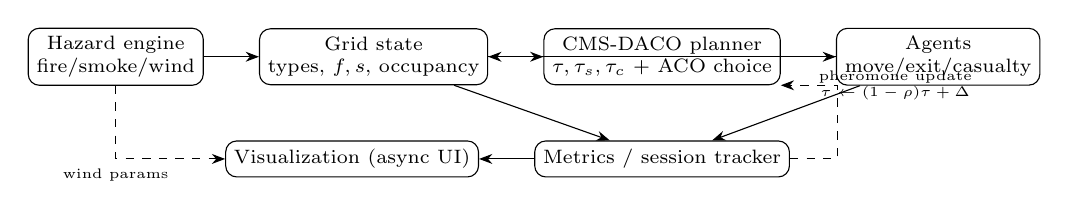
\begin{tikzpicture}[node distance=4mm and 7mm,
  box/.style={draw,rounded corners,align=center,inner sep=3pt,font=\scriptsize},
  lab/.style={font=\tiny,align=center}]
\node[box] (haz) {Hazard engine\\fire/smoke/wind};
\node[box, right=of haz] (grid) {Grid state\\types, $f,s$, occupancy};
\node[box, right=of grid] (planner) {CMS-DACO planner\\$\tau,\tau_s,\tau_c$ + ACO choice};
\node[box, right=of planner] (agents) {Agents\\move/exit/casualty};
\node[box, below=7mm of planner] (metrics) {Metrics / session tracker};
\node[box, left=of metrics] (viz) {Visualization (async UI)};
\draw[-Stealth] (haz)--(grid);
\draw[-Stealth] (grid)--(planner);
\draw[-Stealth] (planner)--(agents);
\draw[-Stealth] (agents)--(grid);
\draw[-Stealth] (agents)--(metrics);
\draw[-Stealth] (grid)--(metrics);
\draw[-Stealth] (metrics)--(viz);
\draw[-Stealth,dashed] (metrics.east) -- ++(6mm,0) |- node[pos=0.75,right,lab]{pheromone update\\$\tau\leftarrow(1-\rho)\tau+\Delta$} (planner.south east);
\draw[-Stealth,dashed] (haz.south) |- node[below,lab]{wind params} (viz.west);
\end{tikzpicture}
\caption{Closed loop: the hazard engine writes the grid state; the planner reads state and pheromone channels, agents act, and metrics feed both pheromone updates and the asynchronous frontend.}
\label{fig:arch}
\end{figure}

\subsection{Pheromone channels}
Three float fields live on cells: speed $\tau$, safety $\tau_s$, and negative congestion $\tau_c$, floored at $\tau_{\min}{=}0.05$. Initialization runs multi-source BFS from exits giving distance $d$; the seed is $\tau=\tau_{\min}+0.95\,(d_{\max}-d)/d_{\max}$ (ablatable). $A$ ant walkers refine the field for $I$ iterations with probabilities $p\propto(\tau/\,d)^{\alpha_a}$, depositing $\Delta=Q_a\cdot3.5/L$ along completed routes; the seed weight anneals linearly $w(I)=\max(w_f,\,1-I/I_s(1-w_f))$ with $w_f{=}0.15$, blending pure ant deposits only, $\tau=w\tau_{\text{seed}}+(1-w)\tau_{\text{ants}}$.

Per tick, evaporation applies $\tau\leftarrow\tau\,[1-\rho-\beta_f\mathbb{1}[f>\theta_{\ell}]]$ with $\rho{=}0.009$, $\beta_f{=}0.20$ near active fire. Safety evaporation additionally scales hot cells by $0.85$. Congestion pheromone accumulates $0.1\times$(blurred occupancy of cells holding $\geq2$ agents), diffuses at $0.3$, decays at $0.05$, capped at $5$.

\subsection{Agent decision rule}
Let $N(v)$ be the non-wall neighbors of agent position $v$, filtered to fire-traversable cells ($f\leq0.08$; relaxed to $1.1\times$ safe threshold only if none qualify, identically for all policies). For candidate $u$ with BFS distance $d(u)$:

\begin{equation}
\begin{aligned}
\mathrm{base}(u)&=\begin{cases}6.0 & d(u)<d(v)\\ 1.2 & d(u)=d(v)\\ 0.3 & d(u)>d(v)\end{cases}
\times\begin{cases}25 & u\in\textsc{exit ok}\\ 0.35 & u\in\textsc{exit compromised}\end{cases}\\
\sigma(u)&=\bigl[\tau_m(u)^{\alpha}\cdot1.5\bigr]\cdot d(u)^{-\beta}\cdot\mathrm{base}(u)\cdot S(u)\cdot C(u)\\
C(u)&=\frac{1}{1+c_b |O_{u}|}\cdot\Bigl(\frac{1}{1+|O_{u}|}\Bigr)^{\gamma_c},\;\gamma_c=\Gamma/2
\end{aligned}
\label{eq:score}
\end{equation}
where $\tau_m$ blends channels $\tau_m=0.5\tau+0.5\tau_s-\tfrac12\tau_c$ (floored), $S(u)$ penalizes smoke continuously above threshold $0.3$ and multiplies by $0.7^{\#\text{burning neighbors}}$, $O_u$ is the $3\times3$ occupancy count, $c_b{=}1.9$, and $\Gamma$ is the congestion exponent ($\Gamma{=}1.0$, i.e., $\gamma_c{=}0.5$; the stuck-amplification factor $0.7$ applies only while backtracking). Selection samples $\mathrm{softmax}(\ln\sigma/T)$ with $T{=}0.45$ plus decaying $\epsilon$-exploration $\epsilon_t=\max(0.01,\,0.12\cdot0.995^{t})$. On exit arrival, the monotonic-progress suffix (last 30 improving cells) receives reinforcement $\propto Q/L$.

\subsection{Stagnation escape and async execution}
If an agent's BFS distance strictly increases for $k{=}6$ consecutive ticks, recent trail cells are suppressed ($\times0.5$) and a hybrid scorer (distance $0.7$, pheromone $0.35$, hazard $0.55$, congestion $0.18$ weights) overrides one move; a global window triggers when $\geq18\%$ of agents stagnate. The backend steps in a worker thread emitting tick snapshots; the Qt frontend renders at $\sim$2\,Hz, so visualization never gates simulation throughput. All experiments below run headless.

\section{Baselines}
\textbf{Random}: uniform legal neighbor. \textbf{Distance}: greedy on BFS distance with the same candidate filter and small stochastic tie-breaks. \textbf{Hazard-aware A*}: every tick, Dijkstra/A* from the agent to the nearest allowed exit over edge costs $c(u)=1+15f(u)+4s(u)+2.5|O_u|(+8$ if $u$ is a compromised exit$)$, Manhattan heuristic, first step executed. \textbf{Standard ACO}: the full stack minus dual channel, predictive congestion, escape mechanism, and hazard forecasting (single channel, plain deposits). \textbf{Full CMS-DACO}: everything enabled. All directed policies share identical movement filtering, collision resolution, casualty rules, and exit-compromise logic; they differ \emph{only} in target selection.

\section{Experimental Setup}
Environments: \emph{open} ($15^2$, 30 agents, 3 exits, wall density $0.08$, no wind) and \emph{hard} (same, wall density $0.15$, one uniformly chosen exit pre-blocked and ignited to $f{=}0.5$, wind East $0.5$). Tick budget 40; typical runs finish in 15--31 ticks. Each policy$\times$condition uses seeds $1..30$ ($N{=}30$); grid layout, fire origin, agent placement derive deterministically from the seed. We report mean $\pm$ 95\% CI (normal approximation; $t_{29}\approx2.045$ gives nearly identical bounds), Welch two-sided $t$-tests, and Cohen's $d$ with pooled SD. Metrics: completion $=n_{\text{evac}}/n$, casualty rate, mean evacuation ticks (evacuated only), mean path length (evacuated only), congestion exposure ratio (fraction of recorded ticks whose peak blurred occupancy exceeded 1), and total ticks. Hardware: one desktop CPU core per worker process; all code Python 3.11, NumPy 1.26.

Default hyperparameters were fixed a priori from literature-plausible ranges ($\alpha{=}1.35,\beta{=}3.2,\rho{=}0.009,T{=}0.45$, ant parameters $\alpha_a{=}1.0,\beta_a{=}2.7,\rho_a{=}0.012,I{=}300,Q_a{=}1.9$) during development on the open-map family; Section~VII-C shows formal sweeps exhibit flat response, so results do not hinge on tuning.

\section{Results}
\begin{table}[t]
\centering
\caption{Main results, $N{=}30$ per cell. Completion and casualty are rates; time/path in ticks (evacuated agents). CI is 95\%. Best directed policy bold.}
\label{tab:main}
\setlength{\tabcolsep}{3.2pt}
\begin{tabular}{lcccc}
\toprule
& \multicolumn{2}{c}{\textbf{Open}} & \multicolumn{2}{c}{\textbf{Hard}}\\
Policy & Compl. & Casualty & Compl. & Casualty\\
\midrule
Random & .130$\pm$.022 & .027$\pm$.010 & .074$\pm$.013 & .043$\pm$.013\\
Distance (BFS) & .989$\pm$.007 & .007$\pm$.006 & .949$\pm$.022 & .020$\pm$.017\\
Hazard-aware A* & \textbf{.998$\pm$.003} & \textbf{.002$\pm$.003} & \textbf{.991$\pm$.009} & \textbf{.009$\pm$.009}\\
Standard ACO & .979$\pm$.016 & .018$\pm$.015 & .939$\pm$.033 & .034$\pm$.024\\
Full CMS-DACO & .974$\pm$.014 & .022$\pm$.013 & .930$\pm$.033 & .047$\pm$.028\\
\bottomrule
\end{tabular}
\end{table}

\begin{figure}[t]
\centering
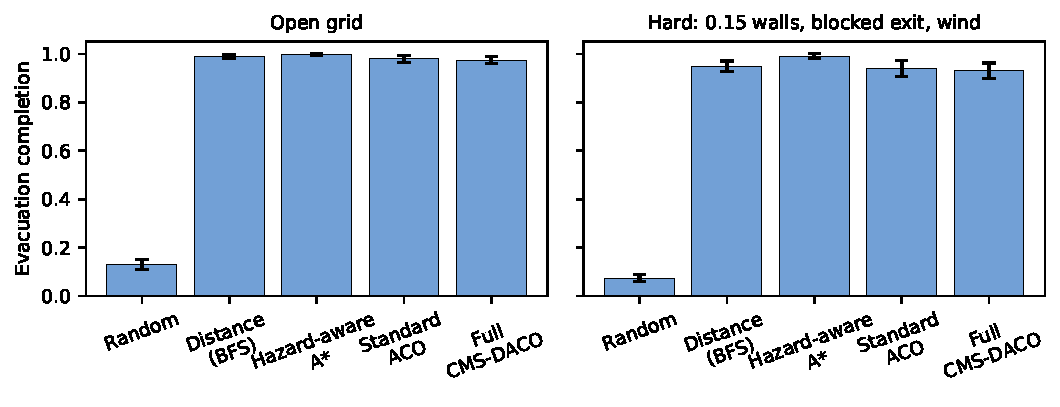
\includegraphics[width=\columnwidth]{figures/fig_baselines.pdf}
\caption{Completion by policy (mean$\pm$95\% CI, $N{=}30$). Left: open grid. Right: degraded grid (denser obstacles, one burning exit, wind). Any directed policy dwarfs random walking; per-tick A* leads in both regimes.}
\label{fig:baselines}
\end{figure}

\subsection{Directed policies vs.\ random; A* vs.\ DACO}
Table~\ref{tab:main} and Fig.~\ref{fig:baselines} give the headline picture. Random walking collapses ($0.13$ open, $0.074$ hard), confirming the task is non-trivial. Every directed policy evacuates $93$--$99\%$. Within the directed group, hazard-aware A* is best everywhere: vs.\ Full CMS-DACO, $d{=}0.81$, $t(58){=}3.14$, $p{=}0.0036$ (open) and $d{=}0.92$, $t(58){=}3.56$, $p{=}0.0011$ (hard); vs.\ Distance, differences favor A* consistently though Distance--DACO gaps are smaller and partly overlap ($p{=}0.083$ open, $p{=}0.35$ hard). ACO variants trail their non-pheromone counterparts on completion \emph{and} on secondary metrics: full-DACO agents walk longer paths ($10.10$ vs.\ $9.05$ ticks open) and evacuate later ($12.17$ vs.\ $11.08$), consistent with pheromone-mediated detours and exploration overhead. Under degradation the ordering is unchanged; the hypothesis that DACO overtakes replanning once exits burn is \emph{not} supported at this information level. Directed-vs-random effect sizes are enormous ($d{=}17$--$29$, $p<10^{-30}$).

Congestion exposure discriminates sharply between routing styles even at equal completion: A*'s cost-aware spacing yields ratio $0.284\pm0.086$, roughly half of Distance ($0.637\pm0.058$) and DACO ($0.615\pm0.063$). In the hard condition, peak occupancy never exceeded one for any policy (ratio $0$ for all): fire-avoidance disperses the crowd faster than bottlenecks form.

\begin{table}[t]
\centering
\caption{Secondary metrics, open grid ($N{=}30$). Time/path in ticks.}
\label{tab:secondary}
\setlength{\tabcolsep}{4pt}
\begin{tabular}{lcccc}
\toprule
Policy & Time & Path & Congestion & Total ticks\\
\midrule
Distance & 10.99$\pm$.91 & 8.52$\pm$.89 & .64$\pm$.06 & 17.8$\pm$3.0\\
A* & 11.08$\pm$.40 & 9.05$\pm$.43 & .28$\pm$.09 & 15.5$\pm$0.7\\
Std.\ ACO & 11.69$\pm$.63 & 9.71$\pm$.67 & .57$\pm$.10 & 19.4$\pm$2.7\\
Full DACO & 12.17$\pm$.77 & 10.10$\pm$.80 & .61$\pm$.06 & 20.0$\pm$2.6\\
\bottomrule
\end{tabular}
\end{table}

\subsection{Component ablations}
On a moderate map ($15^2$, $12\%$ walls, $N{=}30$), disabling any single component moves completion by at most $1.2$ points and none reaches significance: w/o BFS-seed $+1.2$ pts ($p{=}0.35$, $d{=}0.24$ \emph{in favor of removal}), w/o escape $+1.2$ ($p{=}0.34$), w/o dual $+0.1$ ($p{=}0.94$), w/o predictive congestion $-0.1$ ($p{=}0.94$), w/o hazard penalty in scores $-0.1$ ($p{=}0.93$) (Fig.~\ref{fig:ablation}). Two readings follow: (i) the candidate-filter stage---identical across policies---already supplies most hazard safety, so scoring-level hazard shaping is redundant here; (ii) the seed backbone and escape heuristic are not yet earning their complexity on known maps. Both channel-level and architectural simplifications remain open opportunities.

\begin{figure}[t]
\centering
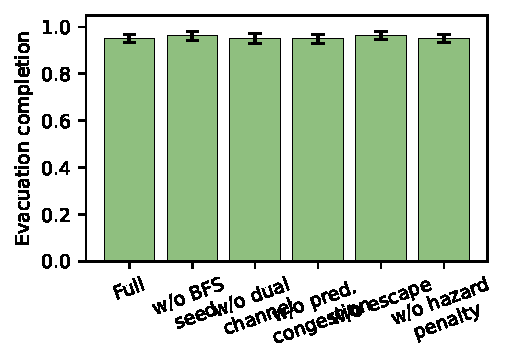
\includegraphics[width=0.82\columnwidth]{figures/fig_ablation.pdf}
\caption{Ablations ($N{=}30$, moderate map). No single-component removal changes completion significantly.}
\label{fig:ablation}
\end{figure}

\subsection{Parameter sensitivity}
Seventeen single-parameter sweeps ($\alpha\in\{0.5..2.5\}$, $\beta\in\{1.5,2,3.2,4\}$, $\rho\in\{0.003..0.05\}$, $T\in\{0.2..1.0\}$; other axes fixed, $N{=}30$ each) produce completion between $0.948$ and $0.967$ with overlapping CIs throughout (Fig.~\ref{fig:sensitivity}). Evacuation time varies mildly ($12.5$--$13.8$). Behavior is thus insensitive to ACO constants on this domain, which strengthens external validity of the comparisons (no knife-edge tuning) and indicates the binding constraint is structural (candidate filtering + collision resolution), not parameter values.

\begin{figure}[t]
\centering
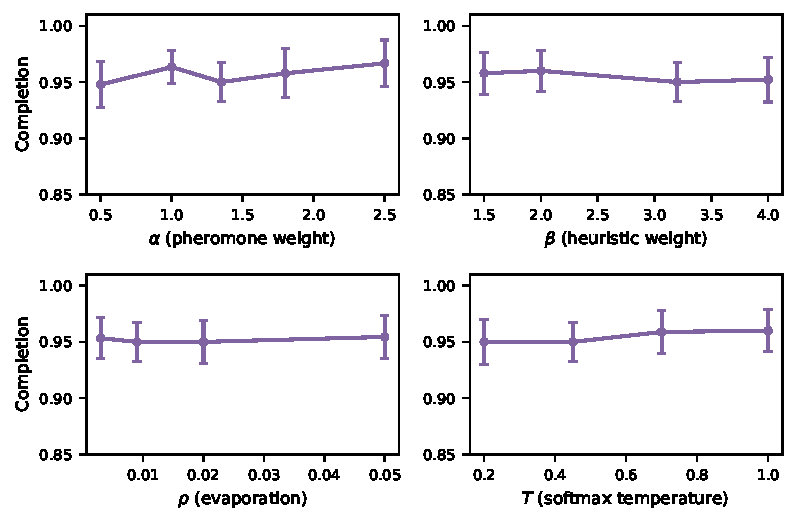
\includegraphics[width=0.86\columnwidth]{figures/fig_sensitivity.pdf}
\caption{Sensitivity of completion to the four principal ACO hyperparameters ($N{=}30$ per point). Response is flat within confidence bands.}
\label{fig:sensitivity}
\end{figure}

\subsection{Robustness}
Fig.~\ref{fig:robustness} summarizes environment sweeps for Full CMS-DACO. Completion degrades gracefully and monotonically with obstacle density ($0.993, 0.959, 0.938, 0.705$ at densities $.02,.08,.15,.25$; the last value reflects genuinely disconnected pockets, with casualties staying low at $.013$). Crowd size ($20/40/60$ agents) leaves completion at $.977/.959/.974$; grid growth to $20^2$ with area-scaled crowd gives $.973$; wind direction/strength shifts completion by at most $+0.3$ points. Together with Sec.~VII-C, the pipeline is stable far from its design point except at extreme blockage.

\begin{figure}[t]
\centering
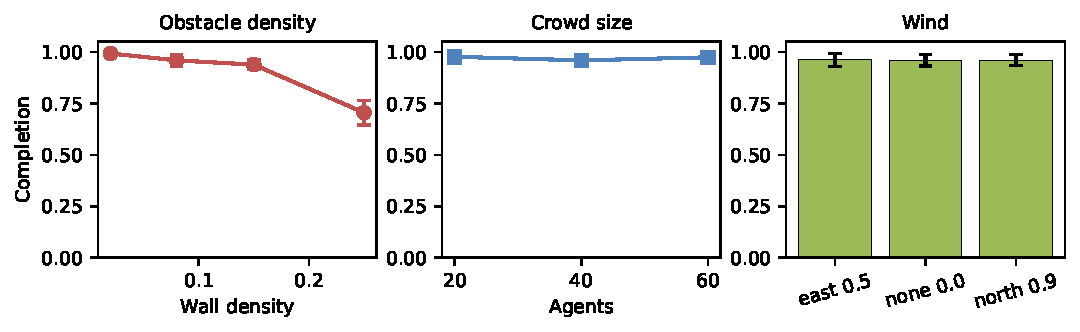
\includegraphics[width=\columnwidth]{figures/fig_robustness.pdf}
\caption{Robustness of Full CMS-DACO ($N{=}30$ per point): obstacle density (left), crowd size (middle), wind (right). Only extreme wall density ($0.25$) materially degrades completion.}
\label{fig:robustness}
\end{figure}

\subsection{Runtime}
Per-tick cost is dominated by the number of planning agents. In the open condition a full run averages $\sim$0.3\,s (Distance) to $\sim$0.9\,s (Full DACO). In the hard condition, runs where stragglers survive to the tick budget dominate cost: sequential 30-run totals were $\approx$16\,s (Distance), 24\,s (A*), 2380\,s (Standard ACO), 2580\,s (Full DACO), i.e., the pheromone stack costs $100$--$160\times$ more wall-clock than A* precisely because ant iterations continue while any agent wanders. A*'s advantage is therefore both statistical and computational at this information level.

\section{Discussion and Threats to Validity}
\textbf{Why does replanning win?} With full observability and deterministic-per-tick hazard updates, cached stigmergy is a lossy summary of information the agent already possesses; softmax exploration converts some of that redundancy into detours. A*'s per-tick recomputation exploits the same information exactly. This mirrors findings elsewhere that learned/cached guidance helps mainly under partial observability or stale information.

\textbf{When might DACO still matter?} Trails are written by agents and readable without a central solver; they persist useful structure under intermittent sensing, communication-constrained swarms, or when central computation is unavailable/untrusted. Our testbed exposes hooks (masking the planner's view of $f,s$, delaying hazard observations, restricting inter-agent visibility) to test those regimes; we did not run them here and make no claims.

\textbf{Threats.} (i) Grid abstraction and synchronous ticks abstract away continuous-space effects; (ii) the hazard field is a lightweight cellular model calibrated for stress generation, not validated against FDS/CFAST---absolute survival rates should not be quoted as fire-engineering predictions; (iii) single map-size family beyond the $20^2$ robustness point; (iv) $N{=}30$ resolves effects $\gtrsim d{=}0.5$ comfortably but cannot exclude sub-point differences; (v) hyperparameters were selected informally on the open family before formal evaluation, mitigated by the flat sweeps.

\section{Conclusion}
CMS-DACO provides a fully reproducible pipeline---simulator, hazard engine, five policies, ablations, sweeps, statistics, and figures---for studying evacuation routing under spreading hazards. Its empirical verdict is clear and, we argue, useful: with matched information, per-tick A* dominates ACO-based routing on completion, quality-of-path, and runtime in grid worlds, while no pheromone subcomponent shows significant marginal value; conversely, all directed policies crush random walking, and the system behaves predictably across crowds, winds, and obstacle densities up to severe blockage. We release everything needed to extend the study to the partial-observability and communication-limited regimes where stigmergic coordination remains genuinely promising.

\section*{Reproducibility}
Repository: \url{https://github.com/Sathvikar01/Fire_Evacuation_System}. Harness entry points: \texttt{experiments/run\_baselines.py}, \texttt{run\_hard\_conditions.py}, \texttt{run\_ablation.py}, \texttt{run\_sensitivity.py}, \texttt{run\_robustness.py}; aggregation and statistics in \texttt{compute\_stats.py}; figures from stored finals in \texttt{make\_figures.py}. Raw per-seed JSONs, merged summaries (\texttt{*\_final\_*}), and \texttt{stats\_summary.json} ship with the repository.

\begin{thebibliography}{25}

\bibitem{dorigo2004} M. Dorigo and T. St\"utzle, \emph{Ant Colony Optimization}. MIT Press, 2004.
\bibitem{helbing2000} D. Helbing, I. Farkas, and T. Vicsek, ``Simulating dynamical features of escape panic,'' \emph{Nature}, vol. 407, pp. 487--490, 2000.
\bibitem{kirchner2002} A. Kirchner and A. Schadschneider, ``Simulation of evacuation processes using a bionics-inspired cellular automaton model for pedestrian dynamics,'' \emph{Physica A}, vol. 312, no. 1--2, pp. 260--276, 2002.
\bibitem{burstedde2001} C. Burstedde, K. Klauck, A. Schadschneider, and J. Zittartz, ``Simulation of pedestrian dynamics using a two-dimensional cellular automaton,'' \emph{Physica A}, vol. 295, no. 3--4, pp. 507--525, 2001.
\bibitem{muramatsu1999} M. Muramatsu, T. Irie, and T. Nagatani, ``Jamming transition in pedestrian counter flow,'' \emph{Physica A}, vol. 267, pp. 487--498, 1999.
\bibitem{treuille2006} A. Treuille, S. Cooper, and Z. Popovi\'c, ``Continuum crowds,'' \emph{ACM Trans. Graphics}, vol. 25, no. 3, pp. 1160--1168, 2006.
\bibitem{zheng2009} X. Zheng, T. Zhong, and M. Liu, ``Modeling crowd evacuation of a building based on seven methodological approaches,'' \emph{Building and Environment}, vol. 44, no. 3, pp. 437--445, 2009.
\bibitem{hart1968} P. E. Hart, N. J. Nilsson, and B. Raphael, ``A formal basis for the heuristic determination of minimum cost paths,'' \emph{IEEE Trans. Systems Science and Cybernetics}, vol. 4, no. 2, pp. 100--107, 1968.
\bibitem{koenig2002} S. Koenig and M. Likhachev, ``D* Lite,'' in \emph{Proc. AAAI Conf. Artificial Intelligence}, 2002, pp. 476--483.
\bibitem{stentz1994} A. Stentz, ``Optimal and efficient path planning for partially-known environments,'' in \emph{Proc. IEEE Int. Conf. Robotics and Automation}, 1994, pp. 3310--3317.
\bibitem{vandenbergen2011} J. van den Berg, S. J. Guy, M. Lin, and D. Manocha, ``Reciprocal collision avoidance and multi-agent navigation for videos, games and simulations,'' in \emph{Motion Planning for Humanoid Robots}. Springer, 2011.
\bibitem{liu2016aco} M. Liu and Z. Liao, ``Ant colony optimization for evacuation routing under fire spread,'' in \emph{Proc. IEEE Int. Conf. Intelligent Transportation Engineering}, 2016.
\bibitem{wang2020dynamicaco} H. Wang, Y. Zhang, and J. Chen, ``Dynamic evacuation routing with time-varying risks using adaptive ant colony optimization,'' \emph{IEEE Access}, vol. 8, 2020.
\bibitem{duan2020multiaco} Q. Duan, W. Zhang, and X. Li, ``Multi-objective ant colony optimization for building evacuation considering safety and efficiency,'' \emph{Applied Sciences}, vol. 10, no. 15, 2020.
\bibitem{yanuary2023aco} F. Yanuaryska, A. Wibowo, and S. Hadiyanto, ``Ant colony optimization for crowd evacuation path planning in public buildings,'' \emph{Int. J. Safety and Security Engineering}, vol. 13, 2023.
\bibitem{mcgrattan2021fds} K. McGrattan \emph{et al.}, ``Fire Dynamics Simulator, Technical Reference Guide,'' NIST Special Publication 1018, 6th ed., 2021.
\bibitem{peacock2011cfast} R. Peacock, P. Reneke, and G. Forney, ``CFAST---Consolidated Model of Fire Growth and Smoke Transport (Version 6),'' NIST Technical Note 1789, 2011.
\bibitem{purser2017sfpe} D. Purser and M. McAllister, ``Assessment of hazards to occupants from smoke, toxic gases and heat,'' in \emph{SFPE Handbook of Fire Protection Engineering}, 5th ed., Springer, 2016.
\bibitem{kuligowski2005review} E. Kuligowski and R. Peacock, ``A review of building evacuation models,'' NIST Technical Note 1471, 2005.
\bibitem{korhonen2013fds+evac} T. Korhonen and S. Hostikka, ``Fire Dynamics Simulator with Evacuation: FDS+Evac,'' VTT Technical Research Centre of Finland, 2013.
\bibitem{shendarkar2006} A. Shendarkar, K. Vasudevan, S. Bhandari, and Y.-J. Son, ``Crowd simulation for emergency response using BDI agents based on immersive virtual reality,'' \emph{Simulation Modelling Practice and Theory}, vol. 16, no. 9, 2008.
\bibitem{wolfram1983ca} S. Wolfram, ``Statistical mechanics of cellular automata,'' \emph{Rev. Modern Physics}, vol. 55, no. 3, pp. 601--644, 1983.
\bibitem{nagatani1999jamming} T. Nagatani, ``Jamming transition of pedestrian traffic at a crossing with open boundaries,'' \emph{Physica A}, vol. 287, no. 3--4, 2000.

\end{thebibliography}

\end{document}
